\documentclass{article}
\usepackage{amsmath}
\usepackage{tikz}
\usetikzlibrary{arrows.meta}

\begin{document}

\begin{figure}[h]
    \centering
    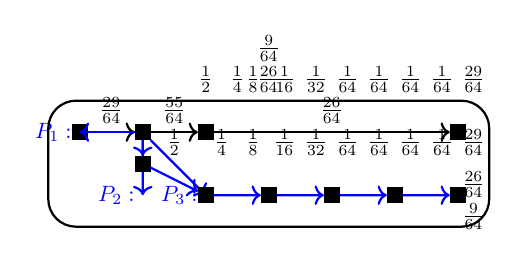
\begin{tikzpicture}[scale=0.8, every node/.style={scale=0.8}]
        % Nodes
        \node (i) at (-3,0) [draw, fill=black] {};
        \node (r) at (-1,0) [draw, fill=black] {};
        \node (r') at (-2,0) [draw, fill=black] {};
        \node (o) at (3,0) [draw, fill=black] {};
        
        % Edges
        \draw[->, thick] (i) -- node[midway, above] {$\frac{29}{64}$} (r');
        \draw[->, thick] (r') -- node[midway, above] {$\frac{55}{64}$} (r);
        \draw[->, thick] (r) -- node[midway, above] {$\frac{26}{64}$} (o);
        
        % Throughput values
        \node at (0,1) [above] {$\frac{9}{64}$};
        \node at (0,0.5) [above] {$\frac{26}{64}$};
        \node at (-1,0.5) [above] {$\frac{1}{2}$};
        \node at (-0.5,0.5) [above] {$\frac{1}{4}$};
        \node at (-0.25,0.5) [above] {$\frac{1}{8}$};
        \node at (0.25,0.5) [above] {$\frac{1}{16}$};
        \node at (0.75,0.5) [above] {$\frac{1}{32}$};
        \node at (1.25,0.5) [above] {$\frac{1}{64}$};
        \node at (1.75,0.5) [above] {$\frac{1}{64}$};
        \node at (2.25,0.5) [above] {$\frac{1}{64}$};
        \node at (2.75,0.5) [above] {$\frac{1}{64}$};
        \node at (3.25,0.5) [above] {$\frac{29}{64}$};
        \node at (3.25,-0.5) [below] {$\frac{26}{64}$};
        \node at (3.25,-1) [below] {$\frac{9}{64}$};
        
        % Lines P1, P2, P3
        \draw[blue, thick, ->] (r') -- ++(-1,0) node[left] {$P_1:$};
        \draw[blue, thick, ->] (r') -- ++(0,-1) node[left] {$P_2:$};
        \draw[blue, thick, ->] (r') -- ++(1,-1) node[left] {$P_3:$};
        
        % Additional nodes for P1, P2, P3
        \node (r1) at (-2,-0.5) [draw, fill=black] {};
        \node (r2) at (-1,-1) [draw, fill=black] {};
        \node (r3) at (0,-1) [draw, fill=black] {};
        \node (r4) at (1,-1) [draw, fill=black] {};
        \node (r5) at (2,-1) [draw, fill=black] {};
        \node (r6) at (3,-1) [draw, fill=black] {};
        
        \draw[blue, thick, ->] (r') -- (r1);
        \draw[blue, thick, ->] (r1) -- (r2);
        \draw[blue, thick, ->] (r2) -- (r3);
        \draw[blue, thick, ->] (r3) -- (r4);
        \draw[blue, thick, ->] (r4) -- (r5);
        \draw[blue, thick, ->] (r5) -- (r6);
        
        % Additional labels for P1, P2, P3
        \node at (-1.5,-0.5) [above] {$\frac{1}{2}$};
        \node at (-0.75,-0.5) [above] {$\frac{1}{4}$};
        \node at (-0.25,-0.5) [above] {$\frac{1}{8}$};
        \node at (0.25,-0.5) [above] {$\frac{1}{16}$};
        \node at (0.75,-0.5) [above] {$\frac{1}{32}$};
        \node at (1.25,-0.5) [above] {$\frac{1}{64}$};
        \node at (1.75,-0.5) [above] {$\frac{1}{64}$};
        \node at (2.25,-0.5) [above] {$\frac{1}{64}$};
        \node at (2.75,-0.5) [above] {$\frac{1}{64}$};
        \node at (3.25,-0.5) [above] {$\frac{29}{64}$};
        
        % Box around the network
        \draw[thick, rounded corners=10pt] (-3.5,0.5) rectangle (3.5,-1.5);
    \end{tikzpicture}
    \caption{A network of size $O(\log q)$ with maximum throughput $\frac{29}{55}$. The throughput values shown on the figure should be scaled by a factor $\frac{64}{55}$ to get the value at equilibrium. The lines $P_1$, $P_2$, $P_3$ are given by the binary encoding of $p = 29 = 011101$, $q = 26 = 011010$ and $2^k - q = 9 = 001001$. \Cref{fig:reversed-optimal-capacity-network} (a) gives another representation of the same network.}
    \label{fig:network-diagram}
\end{figure}

\end{document}